\documentclass{ximera}

\graphicspath{{./}{thePythagoreanTheorem/}{deMoivreSavesTheDay/}{complexNumbersFromDifferentAngles/}{trianglesOnACone/}{cityGeometry/}{EuclidAndGeometry/}}

\usepackage{gensymb}
\usepackage[margin=1in]{geometry}

%\usepackage{hyperref}


\usepackage{tikz}
\usepackage{tkz-euclide}
\usetkzobj{all}
\tikzstyle geometryDiagrams=[ultra thick,color=blue!50!black]
\newcommand{\tri}{\triangle}
\renewcommand{\l}{\ell}
\renewcommand{\P}{\mathcal{P}}
\newcommand{\R}{\mathbb{R}}
\newcommand{\Q}{\mathbb{Q}}

\newcommand{\Z}{\mathbb Z}
\newcommand{\N}{\mathbb N}
\newcommand{\ph}{\varphi}

\renewcommand{\vec}{\mathbf}
\renewcommand{\d}{\,d}



%% Egyptian symbols

\usepackage{multido}
\newcommand{\egmil}[1]{\multido{\i=1+1}{#1}{\includegraphics[scale=.1]{egyptian/egypt_person.pdf}\hspace{0.5mm}}}
\newcommand{\eghuntho}[1]{\multido{\i=1+1}{#1}{\includegraphics[scale=.1]{egyptian/egypt_fish.pdf}\hspace{0.5mm}}}
\newcommand{\egtentho}[1]{\multido{\i=1+1}{#1}{\includegraphics[scale=.1]{egyptian/egypt_finger.pdf}\hspace{0.5mm}}}
\newcommand{\egtho}[1]{\multido{\i=1+1}{#1}{\includegraphics[scale=.1]{egyptian/egypt_lotus.pdf}\hspace{0.5mm}}}
\newcommand{\eghun}[1]{\multido{\i=1+1}{#1}{\includegraphics[scale=.1]{egyptian/egypt_scroll.pdf}\hspace{0.5mm}}}
\newcommand{\egten}[1]{\multido{\i=1+1}{#1}{\includegraphics[scale=.1]{egyptian/egypt_heel.pdf}\hspace{0.5mm}}}
\newcommand{\egone}[1]{\multido{\i=1+1}{#1}{\includegraphics[scale=.1]{egyptian/egypt_stroke.pdf}\hspace{0.5mm}}}
\newcommand{\egyptify}[7]{
 \multido{\i=1+1}{#1}{\includegraphics[scale=.1]{egyptian/egypt_person.pdf}\hspace{0.5mm}}
 \multido{\i=1+1}{#2}{\includegraphics[scale=.1]{egyptian/egypt_fish.pdf}\hspace{0.5mm}}
 \multido{\i=1+1}{#3}{\includegraphics[scale=.1]{egyptian/egypt_finger.pdf}\hspace{0.5mm}}
 \multido{\i=1+1}{#4}{\includegraphics[scale=.1]{egyptian/egypt_lotus.pdf}\hspace{0.5mm}}
 \multido{\i=1+1}{#5}{\includegraphics[scale=.1]{egyptian/egypt_scroll.pdf}\hspace{0.5mm}}
 \multido{\i=1+1}{#6}{\includegraphics[scale=.1]{egyptian/egypt_heel.pdf}\hspace{0.5mm}}
 \multido{\i=1+1}{#7}{\includegraphics[scale=.1]{egyptian/egypt_stroke.pdf}\hspace{0.5mm}}
 \hspace{.5mm}
}




\title{The Pythagorean Theorem}
\begin{document}
\begin{abstract}
In this activity we will prove the most famous theorem of
  all.
\end{abstract}
\maketitle



\begin{question}
Remind us, what is the most famous theorem of all and what exactly
does it assert?
\end{question}


\subsection{Euclid's proof}


\begin{question} 
What would one need to prove about the following diagram to prove the
Pythagorean Theorem?
\begin{image}
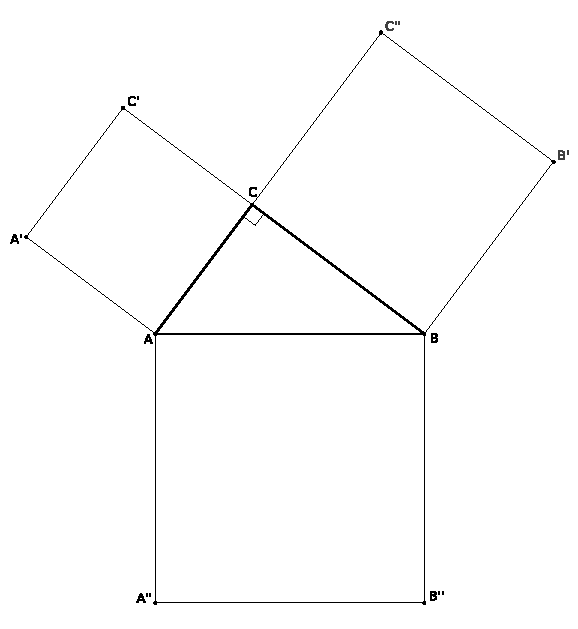
\includegraphics{PythEuclid.pdf}
\end{image}
\end{question}

Let's see if we can do this!


\begin{question}
Draw a line perpendicular to $\overline{AB}$ that passes though both $C$
and $\overline{A'' B''}$. Call the intersection between this line and
$\overline{AB}$, point $E$; call the intersection point between this line
and $\overline{A''B''}$, point $E'$. Explain why $\tri ACA''$ has half the
area of rectangle $AEE'A''$.
\end{question}

\begin{question}
Explain why $\tri ABA'$ has half the area of square $ACC'A'$.
\end{question}

\begin{question}
Explain why $\tri ACA''$ is congruent to $\tri ABA'$. 
\end{question}

\begin{question}
Explain why area of square $ACC'A'$ is equal to the area of rectangle
$AEE'A''$.
\end{question}


\begin{question}
Use similar ideas to complete a proof the Pythagorean Theorem.
\end{question}


\subsection{The converse}

\begin{question} What is the converse to the Pythagorean Theorem? Is it true? How do you prove it?
\end{question}
\end{document}
